% Cap�tulo 3
\chapter{Validation}\label{validationChap}

To validate our guidelines, we searched for open-source tools that could possibly require database transitions. As stated on section \ref{introductionChap}, a database migration is justified when the alternatives have better performance/manutenability than the classic RDBMSs and/or the cost to have a similar performance on the relational database architecture is significantly higher. 


This condition (assessing the need for a database transition) is, then, only verifiable on production or simulated environments. Wordpress\cite{wordpress}, world's most popular Content Management System (CMS)  \cite{cmsranking}, can be used to illustrate this problem.  

Wordpress is built on the top of relational databases, such as PostgreSQL and MySQL. So, to justify a database transition on a wordpress-based application, we must \textit{(i)} have access to a deployed and active version of the CMS or \textit{(ii)} build a simulated environment and load it with posts, pages, comments and other entities that are present on a regular wordpress website.

Having access to the production version of a heavily used tool, such as Wordpress, is not easy, as the owner of the CMS must give access to sensible information of its database, users and posts. 

Other open source tools were considered on this phase of the research, such as Redmine \cite{redmine} and Moodle \cite{moodle}, but the same problem that we had trying to accessing sensible information of Wordpress environments was found on these tools.

Besides that, famous open source tools usually have a large user-base. This results in a large support from the community towards the development of the software. With that, if a database transition from RDBMs to NoSQL is needed, it possibly have plugins/addons from the community, as \cite{fantasticElasticsearch}.

Facing this access restrictions to popular open-seouces projects, to validate the Guidelines proposed on the previous chapter, we have built scenarios that can be easily mapped to real-world applications.

The application proposed on the following section is used on Scenarios 1, 2 and 3, detailed later on this chapter.

\section{Building the Environment}\

To validate the guidelines presented on Chapter~\ref{theProblemChap} we have modeled \textit{the DB Schema core} of an application that gathers posts from social networks and presents them to users. 

Users might use this application to search for relevant topics across Social-Media posts, to classify the subjects of posts, and to build terms cloud and figure out what are the most relevant topics, for example.

From a user perspective, some features of this application are:

\begin{enumerate}
\item{\textbf{Boolean search} - Search posts that mention a boolean query string. \textit{i.e: (Brazil AND Neymar) OR (Orlando AND Kaka)}}
\item{\textbf{Classify posts (add tags)} - \textit{N} tags (subjects) can be added to a single post.}
\item{\textbf{Archive post by query}: A user may archive all posts with a specific characteristic. i.e: it's  possible to archive all posts from 01/01/2015 to 02/01/2015 that have the tag ``Soccer Player''}
\end{enumerate}

Other features of the application are not listed to ease the understanding of the scenarios that are presented on the following sections. 

The database schema was built with the intention of being optimized to production environments, and building \textbf{de}normalized schemas help to leverage application performance, as revealed by \cite{926306}. 

On Figure~\ref{fig:postsTable} it is possible to view all the columns that compose the \textbf{Posts} table. All post entities, like \textit{message} (content of the post), \textit{link} and \textit{number of likes} are present on this table. 

\begin{figure}[ht!]
\centering
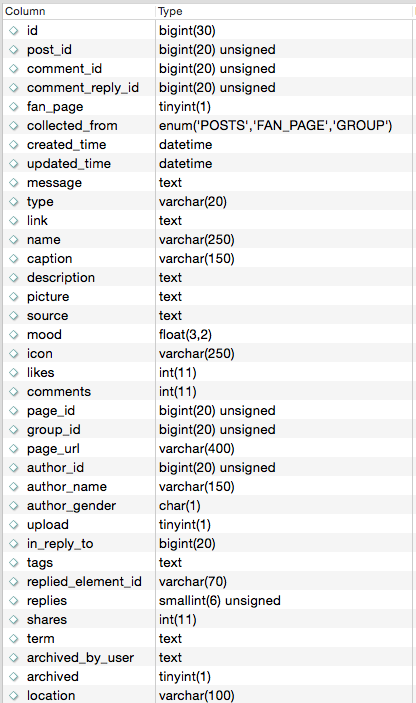
\includegraphics[width=80mm]{postTable.png}
\caption{Posts table.\label{fig:postsTable}}
\end{figure}

On Figure~\ref{fig:tagTable} it is possible to verify the elements that compose a \textbf{Tag} record. Each tag has a unique ID - \textit{idtags}, a \textit{post\_id} (foreign key to the post table), a \textit{tag\_user} (the username of the user who has tagged this post) and \textit{tag\_name}, the subject of this post. 

The Tags table is also denormalized, as \textit{tag\_user} and \textit{tag\_name} are entities that should be represented on separate tables on a normalized schema.

\begin{figure}[ht!]
\centering
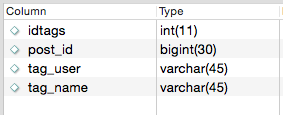
\includegraphics[width=60mm]{tagTable.png}
\caption{Tags table.\label{fig:tagTable}}
\end{figure}

\textbf{Tags} information is purposely redundant. This way, it is possible to retrieve the tags of a post from a \textbf{JOIN} query between the Tags and Post tables and by searching it within the \textit{tags} column of the Posts table. This data-redundancy was planned to test which option has better performance on a production scenario.  


\section{Application SLA}

According to the SLA monitoring-models defined by \cite{ranna2008}, we have defined that a suitable SLA for our application would be a \textit{All-or-nothing}. This way, all the SLOs must be satisfied to gua- rantee that the SLA is still valid.

The SLOs defined on our SLA are: 

\begin{enumerate}
\item{\textit{Search Operation Time:} All search operations must be executed in up to three seconds from the moment that the server receives the request to the moment it sends the response.}
\item{\textit{Search by tags time:} Given an array of tags, the application shoud respond in up to 3 seconds all posts that match this tags array.}
\item{\textit{Update-by-query operations time:} All update-by-query operations should last up to 3 minutes, even if the entire database is updated.}
\end{enumerate}

\section{The application setup}

To prepare our database to the scenarios that will be discussed on the folowing section, some tasks were necessary: 

\subsection{Server Setup}


Setup servers to host the data: A cloud server was needed to host the database that is used on the application. We have selected a \textbf{T2.SMALL} instance from \cite{amazonec2} to host it, as it is a general purpose and low-price instance.

T2.SMALL instances feature the following configuration:

\begin{itemize}
\item{High Frequency Intel Xeon Processors with Turbo up to 3.3GHz Burstable CPU, governed by CPU Credits, and consistent baseline performance}
\item{1 vCPU}
\item{12 CPU Credits/hour}
\item{2 GB RAM}
\end{itemize}

\subsection{Software Setup}
The machine hosted the following software configuration: 

\begin{itemize}
\item{Operating System: Ubuntu 14.04.2 LTS (GNU/Linux 3.13.0-48-generic x86\_64)}
\item{Secure Shell}
\item{MySQL Version: 14.14 Distrib 5.5.44, for debian-linux-gnu (x86\_64) using readline 6.3}
\end{itemize}

\subsection{Data Setup}
To retrieve the data that is used on the scenarios, we have developed a web crawler that gathers posts from Facebook and store them on our MySQL database. 

A total number of 3332534 posts (~ 3 milion posts) were captured and the Dump file with these posts is available on XXXXXXXXXXX. TODO: Upload dump file somewhere. 


\section{Scenario 01}
A possible claim from the application users' is that the Search Speed is slowling down as the number of posts grow in the database. In fact, intuition tells us that the search speed slows down as the number of posts in the database grows. With that, \textit{intuitively} one can say that in some point the first SLO \textit{(Search Operation Time)} will be broken.

To verify this scenario within our database, we have implemented a runnable SLA checker in Python programming language. The algorithm, shown on Figure~\ref{fig:algorithmSLA01} performs fulltext-search operations on our MySQL database and verifies if the SLA is broken in this scenario. 

First, we define several query sizes, and for each query size we generate random strings. Then, a query with of the following style is performed on our MySQL Database: 

 ``SELECT COUNT(*) FROM posts WHERE message like \%myQueryString\%''

For each query size, we repeat the operation with a distinct word for three times (NUMBER\_OF\_ATTEMPTS\_FOR\_EACH\_QUERY\_LENGTH = 3). On our experiments, we found out that there's no noticeable difference between querying random generated ascii-chars and words from the dictionary.

\begin{figure}[ht!]
\centering
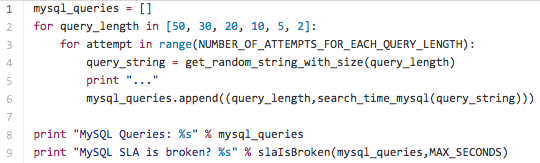
\includegraphics[width=100mm]{algorithmSLA01.png}
\caption{Runnable SLA v0.1 .\label{fig:algorithmSLA01}}
\end{figure}	

We have tested the scenario with [100, 1000,10000, 100000, 100000, 1000000, 2000000 and 30000] posts within our dataset. Execution reports shows us that, indeed, the first SLO is broken with a data-size of 1000000 (one million) posts.

Execution reports for each of these dataset values is available on Appendix B.

\subsection{Guidelines}
The \textbf{first step} of our guidelines states that to propose a database migration, it is necessary to identify that a requirement of the application is broken. In this case, the search speed requirement is broken).

The \textbf{second step} is to implement a runnable SLA that shows that the Service Level Objective is not being fulfilled. The runnable SLA that was explained shows that the Search Operation Time SLO is not being met. 

\textbf{Step number three} is to show that the requirement (or SLO) is broken. Execution Report 01, available on Appendix~\ref{executionreport01} shows that Steps 1, 2 and 3 of our guidelines are done. 

\textbf{The fourth step} of the guidelines is to propose modifications on the relational database. 

TODO finish here. http://blog.scoutapp.com/articles/2014/12/19/from-mysql-full-text-search-to-elasticsearch reporta algumas opcoes para melhorar a performance de um full text search com MySQL. 

Dentre as opcoes para melhorar o processo de search, ele aponta duas solucoes: (i) ``To support full-text search, we needed to use the MySQL MyISAM storage engine. This has major downsides, the primary one being full table locks: when a table is updated, no other changes to that table can be performed.'' A outra saida era (ii) ``We ended up doing this. It was a fairly simple step and allowed us to switch to the InnoDB engine on the master, eliminating the table lock issues.

This bought us some time, but it wasn't a long-term solution: we basically were rolling our own search and this frequently involved complex queries that third-party search libraries could perform more efficiently. We ended up with massive queries composed of many JOINs plus AND/ORs - these aren't easy to maintain.

Besides query complexity, it's tough to beat the performance of a dedicated search solution. Our tables have considerable update activity, so this would result in sometimes-significant performance issues.
''
Outros contra-pontos para implementar fulltext search em MySQL apontado por XXX, XXX and XXX sao X Y e Z. Falta terminar essa parte.

\subsubsection{A new database}

Apache Solr, Lucene, Amazon Cloudsearch and Elasticsearch are \textbf{Search Engines} that provide fulltext-search as master-features. 

Elasticsearch (a.k.a. Elastic) was seemed to be a good alternative to the problem that we were facing with MySQL. Some discussion forums were consulted and comparisons and studies were considered on our research \cite{StackOverflowElastic} \cite{SolrVsES} \cite{quoraES}. With that, \textbf{step number four} is done. 

\textbf{Step number five} suggests that a new data model should be proposed once the new database technology is chosen. As Elasticsearch stores data as JSON documents, the same structure of post that we had on the posts table was transformed into a valid JSON document.

A new server with the same configuration of the one presented on the beginning of this chapter was provisioned and Elasticsearch[1.7.2] version was installed.

To dump the data from MySQL and import to Elasticsearch, a Python script was made \cite{mysqltoes}. However, loading data was taking too long as the script didn't paralellize the bulk insert queries on Elasticsearch and database connection kept dropping. To overcome this situation,an open-source project that connects to MySQL via JDBC and imports data into Elasticsearch \cite{elasticjdbc} was used. 
With that, \textbf{the sixth step} is successfully executed. 

A new runnable SLA was necessary to compare the execution time of the previous database architecture (MySQL) and the one that was proposed. We have joined both runnable SLAs into a single script, available on \cite{runnablesla01}, \textbf{finishing the seventh step}.

It is possible to compare the Execution Report of both database architectures on Execution Report 02 (Appendix \ref{executionreport01}).

With that, it is possible to show that the runnable SLA on the new architecture with all posts results in a significant performance improvement, proving that a database transition may be suitable to this scenario, \textbf{finishing Step 08}.

To proceed with a DB migration, Scenarios 02 and 03 must also be analyzed. 

\section{Scenario 02}
Scenario 02 was searching for an unstructured  document (a tag defined by a user, for example). Shows that even with joins is a costy operation and filling it in a text drives us to a Fulltext-search scenario. 

TODO: everything

\section{Scenario 03}
Update by query scenario

Todo: everything 



% Elasticsearch wins.
%  % Teste para abreviatura 

% \abrv[UFRN -- Universidade Federal do Rio Grande do Norte]{UFRN}

% \section{Scenario 03}
% Update by query Scenario. 

% Elasticsearch doesn't support natively. 

% Update by query plugin

% MySQL wins

% Dizer tamb�m que o pessoal recomenda migrar peda�os de feature a feature, como nesse case do Coursera. https://tech.coursera.org/blog/2014/09/23/courseras-adoption-of-cassandra/
